\hfill\small{11 Jan 2024}
\vspace{0.5em}
\hrule
\vspace{-0.5em}
\section{Lecture 3 --- Linearization}
\subsection{Linearization}

Consider a non linear system \(\dot{x} = f(x)\) with an equillibrium point \(x^{\star} = 0\).
Then using first order Taylor series expansion, we have:
\[
    \dot{x} = f(x) = f(0) + \left . \frac{\partial f}{\partial x} \right |_{x=0} x + \mathcal{O}(x^2)
\]

Thus, the linearised system can be written as:
\[
    \dot{x} = A x \quad \text{where} \quad A = \left . \frac{\partial f}{\partial x} \right |_{x=0}
\]
The matrix \(A\) is called the \emph{Jacobian} of the system \(\dot{x} = f(x)\) evaluated at the
equillibrium point \(x^{\star} = 0\). The system can also be calculated for an equillibrium point
not at origin, by shifting the origin to the equillibrium point.
    
\subsubsection{Pertubations of the eigenvalues}
The study of the behaviour of linear systems about the equillibrium point \(x=0\) is important
beacuse in many cases the behaviour of a nonlinear systems, near an equillibrium point can
be deduced by linearsing the system about the equillibrium point.

The validity and the accuracy of the linearization of the nonlinear system, and the resultant
qualitative behaviour depends on the placement of the eigenvalues of the linearised system.
This can be understood by considering the linear pertubations. Let the linearized system be
given by \(\dot{x} = Ax, x\in\mathbb{R} \), with distinct eigenvalues, and let
\(\Delta A \in \mathbb{R}^{2\times 2}\) be a small pertubation matrix, whose elements have arbitrary
small magnitudes. We know, that the eigenvalues of the matrix \(A + \Delta A\)
depend continuously on the parameters of the matrix. 

Thus, when the matrix \(A\) is pertubed by \(\Delta A\), any eigenvalues of A that lies in
the left or the right half plane, wil remain in its respective half plane. But, the eigenvalues
on the imaginary axis, when perturbed might go into either the left or the right half plane.

Consquently, we can say that if the equillibrium point \(x=0\) of \(\dot{x} = Ax \) is a
node, focus, or saddle, then the equillibrium point \(x=0\) of \(\dot{x} = (A + \Delta A) x \)
will be of the same type, provided that the pertubations are small enough. This situation is quite different in the case of center. Since the qualitative behaviour of the
stable focus and unstable focus are different from that of a center, the center equillibrium 
point will not persist under pertubations.

The node, focus, and saddle equillibrium point are said to be \emph{structurally stable} because they
maintain their qualitative behaviour under infinitesimally small pertubations.

\begin{definition}[Hyperbolic Equillibrium Point]
    An equillibrium point of the system \(\dot{x}= f(x)\) with \(f(x^{\star}) = 0\) is said to be
    hyperbolic if:
    \[
        \Re \left(
            A = \left . \frac{\partial f}{\partial x} \right |_{x=x^{\star}}
        \right) \neq 0
    \] 
    i.e. the jacobian of the system evaluated at the equillibrium point has no eigenvalues
    with zero real part.
\end{definition}

\begin{example}
    Consider the system \(\dot{x} = x^3 , x\in\mathbb{R} \)
    The system has its only equillibrium point at \(x^{\star} =0\). The phase portrait of the system
    is given by:
    \begin{center}
        \begin{tikzpicture}
            % Axis lines
            \draw[-] (-2,0) -- (2,0) node[below right] {$x$};
            
            % Arrows pointing towards each other
            \draw[<->] (1,0) -- (-1,0) node[midway]{};
            
            % Origin point
            \draw[] (0,-0.1) -- (0,0.1);
            \node[below right]{$0$};
        \end{tikzpicture}
    \end{center}
    linearsing the system we have \(\dot{x} = 3x^2 \implies \dot{x} = 0 \).
    
    Thus we can say that for any arbitrary point close to the equillibrium point, the behaviour
    described by the linear system is different from the non linear system
\end{example} 
\begin{example}
    Consider the system given by:
    \[
        \begin{aligned}
            \dot{x}_1 &= -x_2 -\mu x_1 (x_1^2 + x_2^2)\\
            \dot{x}_2 &= x_1 - \mu x_2 (x_1^2 + x_2^2)
        \end{aligned}
    \]
    The system has an equillibrium point at \(x^{\star} = 0\).
    Linearsing the system around the origin we have:
    \[
        A = \left . \frac{\partial f}{\partial x} \right |_{x=0} = \begin{bmatrix}
            0 & -1 \\
            1 & 0
        \end{bmatrix} \implies \lambda = \pm i
    \]
    Note that the linearised system corresponds to a simple harmoic oscillator
    
    Shifting, into polar coordinates to analyse the system, we have:
    \[
        r\coloneqq \sqrt{x_1^2 + x_2^2} \quad \theta \coloneqq \arctan \left( \frac{x_2}{x_1} \right)
    \]
    After some simplification, we have:
    \[
        \dot{r} = -\mu r^3 \quad \dot{\theta} = 1 
    \]
    Depending upon the value of \(\mu\), we have the following:
    \[
        \begin{aligned}
            \mu > 0 &\implies \text{Stable Focus} \\
            \mu = 0 &\implies \text{Center} \\
            \mu < 0 &\implies \text{unstable Focus} \\
        \end{aligned}  
    \]
    Thus, the qualitative behaviour is same for the linearised system and the nonlinear system,
    only at \(\mu = 0\), which can also be trivally observed from the state equations.
\end{example}
Thus, we have a sufficient condition for the qualitative behaviour of the nonlinear system to be
same as the linearised system, which is that the equillibrium point of the nonlinear system should
be hyperbolic.

\begin{theorem}[Hartman-Grobman Theorem]
Let \(\dot{x}=f(x),\:x\in\mathbb{R}^n\) be a nonlinear system with an hyperbolic
equillibrium point \(x_e\). Let \(\phi_t^f\) be the flow map for \(\dot{x}=f(x)\) i.e. \(\dot{x}=f(x),\:x(0)=x_0\)
has the solution \(x(t)=\phi_t^f(x_0)\). Then for a \(\delta >0\) and a ball \(B_{\delta}(x\in\mathbb{R}^n \vert
\Vert x-x^{\star}\Vert < \delta)\) there exits as map \(F : B_{\delta} \subset \mathbb{R}^n \to \mathbb{R}^n, \: \exists T > 0\)
such that, 
\[
    F(x_e) = 0, \text{ F is one to one on } B_\delta \text{ onto } F(B_\delta)  
\]        
and both \(F\) and \(F^{-1} \) exits and are continuous, such that \(F(\phi_t^f) = e^{At}F(x) \forall \vert t \vert
< T\). Where \(A = \left . \frac{\partial f}{\partial x} \right |_{x=x^{\star}}\) and \(x\in B_\delta \)\\

\begin{tikzpicture}
    \node[label=below:$x_0$]  (x0) at (-0.1,1)  {$\bullet$};
    \node[label=below:$x(t)$]  (xt) at (0.5,2)  {$\bullet$};
    \node[label=below:$F(x_0)$]  (Fx) at (6,1)  {$\bullet$};
    \node[label=right:$e^{At}F(x_0)$]  (eAF) at (9,4)  {$\bullet$};
    \draw (0,1.5) circle (1.0) ;
    \node[label=left:$x_e$]  (xe) at (-0.75,1.45)  {$\bullet$};
    \draw (x0.center) to [out=5,in=-90]++(0.25,1.1) to[out=15,in=-95](xt.center); %% in the ball
    % \draw (Fx.center) to [out=10,in=-110]++(2.6,2) to[out=70,in=-103](eAF.center); %%
    \draw (Fx.center) to [out=15,in=-105](eAF.center);
    \begin{scope}[dashed,decoration={
        markings,
        mark=at position 0.5 with {\arrow{>}}}
        ] 
    \draw[postaction={decorate}] (x0.center) to [out=10,in=-520](Fx.center); %%
    \draw[postaction={decorate}] (xt.center) to [out=10,in=-150](eAF.center); %%
    \draw[postaction={decorate}] (eAF.center) to [out=150,in=10](xt.center); %%
    \node at (3,0.25) {$F$};
    \node at (4.75,2.25) {$F$};
    \node at (4.5,3.25) {$F^{-1} $};eAF.center
    \end{scope}
\end{tikzpicture}
\label{thm:hartmanGrobman}
\end{theorem}
\vspace{0.5em}

The map \(F\) in \autoref{thm:hartmanGrobman} maps from the nonlinear world to the linear world. 
\subsubsection{Pendulumn}
One example of periodicity in phase portraits is given by the pendulumn. 
This type of periodic behaviour is not found in linear systems.
\begin{example}[Pendulumn]
    Consider a pendulumn, with normalised dynamics given by:
    \[
        \begin{aligned}
            \dot{x}_1 &= x_2  \\
            \dot{x}_2 &= -\sin(x_1) - x_2
        \end{aligned}
    \]
    The equillibrium points of this system are given by:
    \[
        x_1 = k\pi \quad x_2 = 0 \quad k\in\mathbb{Z}
    \]
    Calculating the jacobian of the system, we have:
    \[
        A = \left . \frac{\partial f}{\partial x} \right |_{x=x^{\star}} = \begin{bmatrix}
            0 & 1 \\
            -\cos(x_1) & -1
        \end{bmatrix}
    \]
    Evalating the jacobian at \((0,0)\) and \((\pi,0)\) we have :
    \[
        \begin{aligned}
            \left. \frac{\partial f}{\partial x} \right |_{x=(0,0)} &= \begin{bmatrix}
                0 & 1 \\
                -1 & -1
            \end{bmatrix} \implies \lambda = \frac{-1 \pm \sqrt{3}}{2} \\
            \left. \frac{\partial f}{\partial x} \right |_{x=(\pi,0)} &= \begin{bmatrix}
                0 & 1 \\
                1 & -1
            \end{bmatrix} \implies \lambda = \frac{-1 \pm \sqrt{5}}{2} \\
        \end{aligned}
    \]
    The phase portrait of the system is given by:
    \begin{center}
        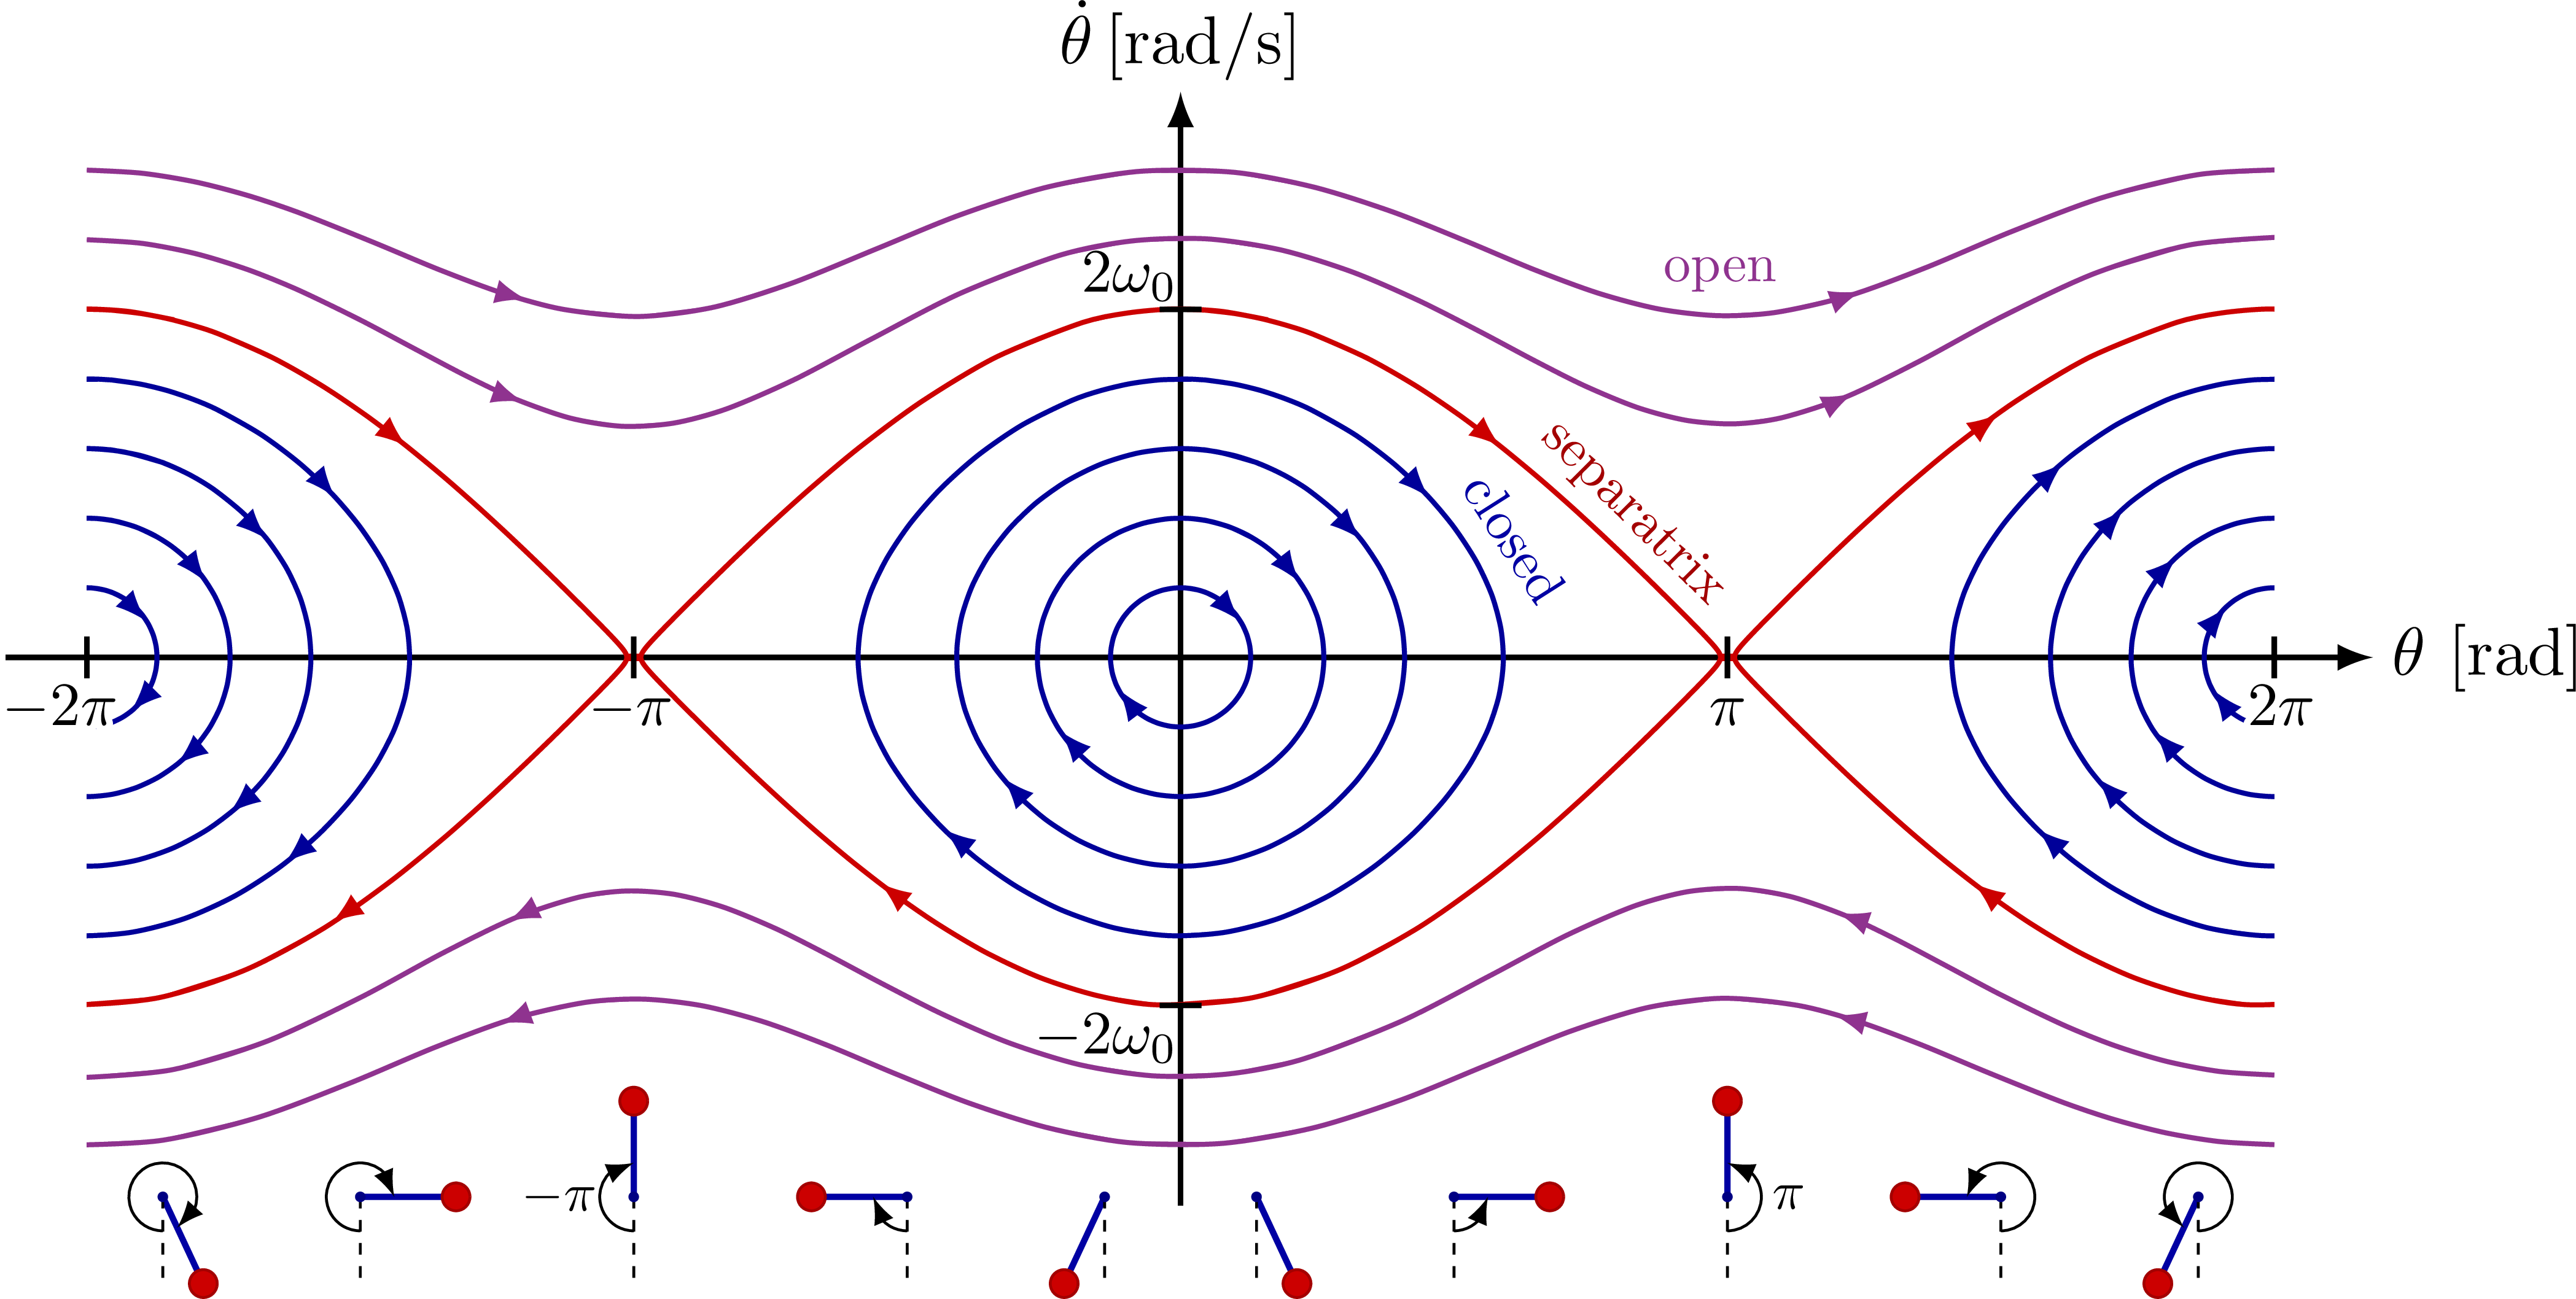
\includegraphics[width=\linewidth]{figures/phaseportraits/pend.png}
    \end{center}
    The image source is \href{https://tikz.net/dynamics_phaseportrait/}{linked here}
\end{example}




